\section{Projeto de controladores por \textit{negative feedback}}


\subsection{Método do lugar das raízes}

\subsubsection{Projeto do Controlador}

\begin{comment}
O sistema em malha aberta dado, ao qual seria preciso melhorar o seu desempenho foi:

\begin{equation}\label{planta:eq}
    G_p(s) = \frac{2}{s(s+0,5)}
\end{equation}
\end{comment}


O desempenho escolhido para o sistema foi de $e.r=0$ para $r(t)=1$, $T_{S2\%}  \leq 2s$ e $PO \% \leq 5\%$.

Inicialmente foi analisada a planta e notou-se que ela já satisfazia o requisito de erro em regime, pois já existia um componente integrador no sistema, garantindo assim o erro em regime nulo. Posteriormente, foi checado o tempo de estabilização, que inicialmente era de 16 segundos. Para que o tempo seja menor ou igual a 2 segundos, temos que satisfazer a equação  $T_{S2 \%} = \frac{4}{\xi w_n}$, que nos dá que $\xi w_n = 2$. Dessa forma, teremos a parte real dos polos em $-\xi w_n = -2$. No potencial de \textit{overshoot}, temos associado ao de $5\%$, um coeficiente de amortecimento $\xi = 0,7$ e um ângulo $\theta = 45\degree$, mostrando assim que teremos um par complexo conjugado nos polos.

Com essas considerações, chegamos a conclusão que usaremos um controlador proporcional derivativo, PD. Sua equação padrão é:
\begin{equation}
    G_c(s) = K_c\tau_d\left(s+\frac{1}{\tau_d}\right)
\end{equation}

Com isso, encontraremos $K_c$ e $\tau_d$ satisfazendo as duas condições do lugar das raízes, a condição angular e a condição de magnitude. A condição angular nos diz que o somatório dos ângulos dos polos e zeros, no conjunto controlador+planta, no lugar das raízes tem que ser igual a $180\degree$. Assim, temos:

\begin{equation}
    \phase{A(s_i)} = 180\degree, \forall s_i \in RL
\end{equation}
Como temos dois polos na planta e teremos um zero adicionado pelo PD, a equação fica:
\begin{center}
    $\phase{A(s_i)} = \theta_Z - \theta_P_1 - \theta_P_2 = 180\degree$
\end{center}
É possível encontrar $\theta_P_1$ e $\theta_P_2$ por meio dos parâmetros dados. Sabemos que $s_i$ vale $-2$ no eixo real e tem ângulo $45\degree$ com a origem. Como $\theta_P_1$ se encontra na origem, temos:
\begin{center}
    $\theta_P_1 = 180\degree - 45\degree = 135\degree$
\end{center}
Já $\theta_P_2$ se encontra em $-0,5$ no eixo real. Podemos encontrar seu valor usando um arco tangente, pois como o ângulo de $s_i$ é $45\degree$, seu valor no eixo imaginário é igual ao seu valor no eixo real. Logo, temos:
\begin{center}
    $\theta_P_2 = 180 - arctg\left(\frac{2}{1,5}\right) = 126,87\degree$
\end{center}
Assim, podemos encontrar o valor de $\theta_Z$:
\begin{center}
    $\theta_Z - \theta_P_1 - \theta_P_2 = 180\degree$ \vspace{5pt}\\
    $\theta_Z = 180\degree + \theta_P_1 + \theta_P_2$ \vspace{5pt}\\
    $\theta_Z = 180\degree + 135\degree + 126,87\degree$ \vspace{5pt}\\
    $\theta_Z = 441,87\degree = 81,87\degree$ \vspace{5pt}
\end{center}
Com o valor de $\theta_Z$, podemos calcular o valor do zero do PD no lugar das raízes. Considerando "d" a distancia entre $s_i$ e o zero, temos:
\begin{center}
    $tg(81,87\degree) = \frac{2}{d}$ \vspace{5pt}\\
    $d = \frac{2}{tg(81,87\degree)}$ \vspace{7pt}\\
    $d = 0,286$
\end{center}
Como d é apenas a distancia entre $s_i$ e o zero, para encontrar o $\tau_d$, somaremos com $-2$:
\begin{center}
    $-\frac{1}{\tau_d} = -2 - 0,286$ \vspace{5pt}\\
    $\tau_d = \frac{-1}{-2,268}$ \vspace{5pt}\\
    \boxed{\tau_d = 0,437}
\end{center}
Agora nos resta checar a condição de magnitude. Ela nos diz que o módulo dos zeros e polos, do conjunto controlador+planta, tem que ser igual a 1. Assim, temos:
\begin{equation}
    |A(s_i)| = 1, \forall s_i \in RL
\end{equation}

Teremos então, na equação, a amplitude do zero e dos dois polos, além dos valores de ganho $K_c$, de $\tau_d$ e o ganho que já estava na planta. Temos, então:
\begin{center}
    $|A(s_i)| = 1$ \vspace{7pt}\\
    $\frac{2 K_c \tau_d A_Z}{A_P_1 A_P_2} = 1$ \vspace{7pt}\\
    $K_c = \frac{A_P_1 A_P_2}{2 \tau_d A_Z}$
\end{center}
Para encontrar os valores de amplitude, basta apenas encontrar as distancias dos polos e zeros para o $s_i$. Logo:
\begin{center}
    $K_c = \frac{A_P_1 A_P_2}{2 \tau_d A_Z}$ \vspace{7pt}\\
    $K_c = \frac{\sqrt{2^2 + 2^2}*\sqrt{2^2 + 1,5^2}}{2*0,437*\sqrt{2^2 + 0,286^2}}$ \vspace{7pt}\\
    \boxed{K_c = 4,00}
\end{center}

Assim, o PD fica da seguinte forma:
\begin{center}
    $G_c(s) = 4,00*0,437\left(s+\frac{1}{0,437}\right)$ \vspace{7pt}\\
    \boxed{G_c(s) = 1,748(s+2,286)}
\end{center}

Com a inserção do controlador no sistema, temos um novo zero no lugar das raízes, de forma a modificá-lo. Nas figuras ~\ref{xcos:rl:a} e ~\ref{xcos:rl:b} é possível ver a diferença. Foi utilizado a função \textbf{evans()} do \textbf{Scilab} para obter esses gráficos. Os quadrados por cima da linha do lugar das raízes na figura ~\ref{xcos:rl:b} mostram exatamente os novos polos do sistema.

\begin{figure}[H]
\begin{center}
    \subfigure[Lugar das raízes da planta]{             
        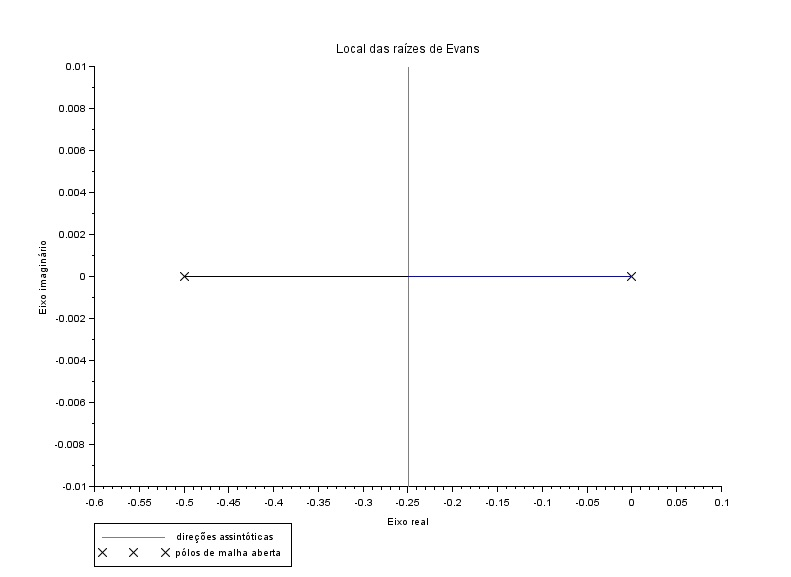
\includegraphics[width=7.75cm]{images/metodo_rl/old_rl.jpg}  
        \label{xcos:rl:a}
    }
    \subfigure[Lugar das raízes da planta+controlador ]{ 
        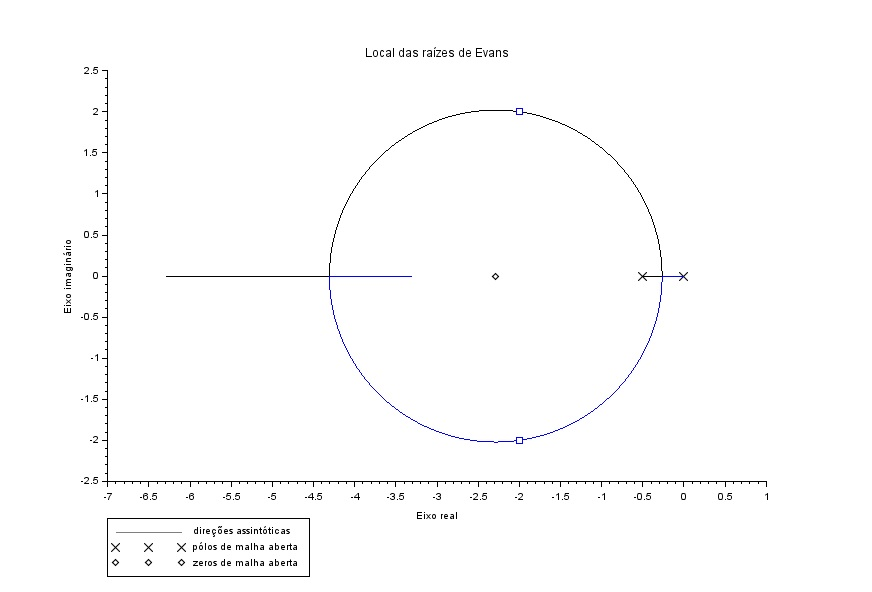
\includegraphics[width=7.75cm]{images/metodo_rl/new_rl.jpg}
        \label{xcos:rl:b}
    }                
\end{center}
\caption{Simulação com o sistema planta+controlador em malha fechada no XCOS.}
\label{xcos:rl} 
\end{figure}

\subsubsection{Simulações no Scilab}

Com os parâmetros obtidos no projeto, é feita a análise comparativa dos mesmos a partir da simulação. Neste caso, foi usada a ferramenta de modelagem e simulação de sistemas \textbf{XCOS}, incluso no software \textbf{Scilab}, que conta com diagrama de blocos ajustáveis de mais variadas funções úteis à realização do sistema.

Ao anteriormente explanado sistema em malha fechada foi integrado o controlador PD gerado com o método do lugar das raízes, com a finalidade atender adequadamente aos requisitos de desempenho. As Figuras ~\ref{xcos:mrl:a} e ~\ref{xcos:mrl:b} abaixo mostram, respectivamente, a modelagem e simulação do sistema. O bloco PID da Figura ~\ref{xcos:mrl:a} é, funcionalmente, um controlador PD e teve de ser mantido assim por limitações do software.


\begin{figure}[H]
\begin{center}
    \subfigure[Diagrama de blocos]{             
        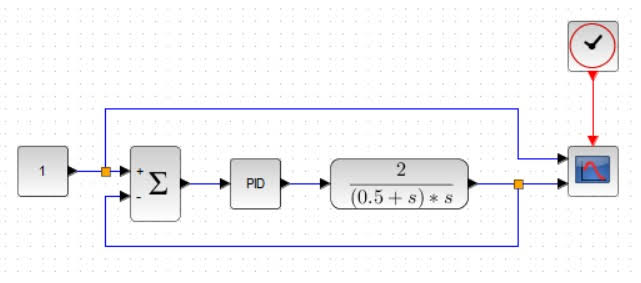
\includegraphics[width=6cm]{images/metodo_rl/diag_mrl.jpg}  
        \label{xcos:mrl:a}
    }
    \subfigure[Simulação temporal]{                                              
        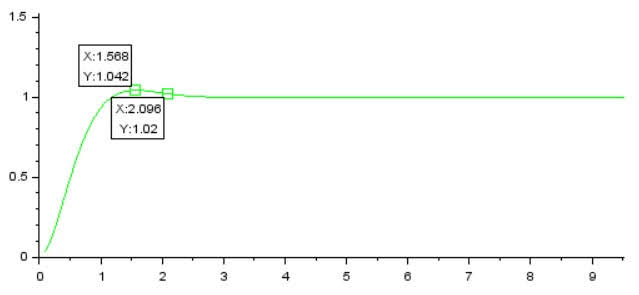
\includegraphics[width=9.5cm]{images/metodo_rl/time_mrl.jpg}
        \label{xcos:mrl:b}
    }                
\end{center}
\caption{Simulação com o sistema planta+controlador em malha fechada no XCOS.}
\label{xcos:mrl} 
\end{figure}

Observa-se um percentual de \textit{overshoot} de $4,5\%$ e um tempo de estabilização de $2\%$ de 2,096 segundos. Tais parâmetros se aproximam dos resultados teóricos e, embora haja uma ultrapassagem pequena no tempo de estabilização, este valor está dentro de uma margem de aceitabilidade. É válido lembrar que o desempenho quanto ao erro em regime permanente já havia sido atendido antes mesmo do uso do controlador.

\subsection{Método polinomial}

\subsubsection{Projeto do Controlador}

\begin{comment}
O sistema dado pelo docente da disciplina em malha aberta foi:

\begin{equation} \label{plant:eq}
    G_p(s) = \frac{2}{s(s+0,5)}
\end{equation}
\end{comment}


Estabeleceu-se o desempenho desejado para o sistema para $e.r=0$ para $r(t)=1$, $T_S_2_\% \le 4s$ e $PO\% \le 5\%$.

Então, primeiramente, antes de iniciar os devidos cálculos, observou-se os requisitos para se atender no limiar o desempenho desejado para o sistema. Para o erro em regime, como a planta já possui um componente integrador, já existe a garantia da anulação do erro em regime. Para o percentual de \textit{overshoot}, por tabela, associa-se a um $\xi = 0.7$ e, consequentemente, $\theta = 45\degree$, sendo assim, já se percebe a necessidade de um par de polos complexos conjugados. Quanto ao tempo de estabilização, para se atender o tempo de 4 segundos, pela equação $T_S_2_\% = \frac{4}{\xi w_n}$, necessita-se de polos com parte real ($-\xi w_n$) igual a -1.

Diante disto, para atender o desempenho desejado para o sistema, será necessário que a combinação controlador+planta em malha fechada tenha os pólos $-1 \pm j1.020$. Ou seja, o denominador da função de transferência em malha fechada, deve conter $s^2 + 2s + 2.041$. Sendo assim, partiu-se para a projeção, de fato do controlador, utilizando o método polinomial, baseado na equação diofantina.

A partir das inequações dos graus dos polinômios para aplicação do método, pode-se assumir as igualdades abaixo:

\begin{center}
    $n_a_* \ge n_a = 2 \Rightarrow n_a_* \ge 2 \Rightarrow$ \boxed{n_a_* = 2} \vspace{5pt}\\
    $n_l \le máx(n_a_* - n_a, n_b - 1) = máx(0, -1) \Rightarrow n_l \le 0 \Rightarrow$ \boxed{n_l = 0} \vspace{5pt}\\
    $n_p < n_a \Rightarrow n_p < 2 \Rightarrow$ \boxed{n_p = 1} \vspace{5pt}
\end{center}

A partir dos graus assumidos nas expressões acima, pode-se destacar o formato dos polinômios conforme abaixo:

\begin{center}
    $a^*(s) = s^2 + 2s + 2.041$ \vspace{5pt}\\
    $b(s) = 2$ \vspace{5pt}\\
    $a(s) = s^2 + 0.5s$ \vspace{5pt}\\
    $\rho(s) = \rho_1s + \rho_0$ \vspace{5pt}\\
    $l(s) = l_0$ \vspace{5pt}
\end{center}

Neste ponto, aplicou-se a equação diofantina $a^*(s) = a(s)l(s) + b(s)\rho(s)$. Então, resolvendo-a, obteve-se:

\begin{center}
    \boxed{l_0 = 1} \vspace{5pt}\\
    $0.5l_0 + 2\rho_1 = 2 \Rightarrow$ \boxed{\rho_1 = 0.75} \vspace{5pt}\\
    $2\rho_0 = 2.041 \Rightarrow$ \boxed{\rho_0 = 1.021} \vspace{5pt}
\end{center}

Sendo assim, a função de transferência do controlador encontrada foi equivalente a um controlador do tipo PD, como segue abaixo:

\begin{center}
    $G_c(s) = 0.75s + 1.021 \Leftrightarrow$ \boxed{G_c(s) = 0.75(s + 1.361)} \vspace{5pt}
\end{center}

\subsubsection{Simulações no Scilab}

A partir dos cálculos realizados, partiu-se para as simulações com o fim de se visualizar o comportamento do sistema em três situações: planta em malha aberta, planta em malha fechada e sistema planta+controlador em malha fechada. Sendo que as duas primeiras simulações já foram inicialmente explicitadas. Para as simulações, utilizou-se a ferramenta disponível no software livre \textbf{Scilab} chamada \textbf{XCOS}, com a qual é possível construir o diagrama de blocos e parametrizá-los de forma bem simples. Assim, segue-se.

Adicionou-se o controlador obtido através do método polinomial com o sistema em malha fechada, como mostra o diagrama da Figura ~\ref{xcos:mfc:a} e, assim, obteve-se a saída conforme a Figura ~\ref{xcos:mfc:b}, apresentando um percentual de \textit{overshoot} de aproximadamente $4.5\%$ e tempo de estabilização em torno de $4.18$ segundos.

\begin{figure}[H]
\begin{center}
    \subfigure[Diagrama de blocos]{             
        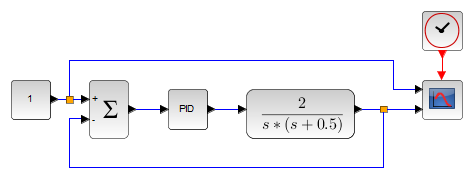
\includegraphics[width=6cm]{images/metodo_polinomial/diag_mfc.png}  
        \label{xcos:mfc:a}
    }
    \subfigure[Simulação temporal]{                                              
        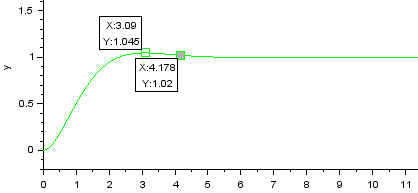
\includegraphics[width=9.5cm]{images/metodo_polinomial/time_mfc.png}
        \label{xcos:mfc:b}
    }                
\end{center}
\caption{Simulação com o sistema planta+controlador em malha fechada no XCOS.}
\label{xcos:mfc} 
\end{figure}

Sendo assim, a partir destas simulações, percebe-se que o controlador projetado atende ao desempenho desejado inicialmente para a planta, com certa imprecisão no tempo de estabilização, mas isto é normal em virtude dos arredondamentos e, além disso, admite-se que o desempenho requerido já possui uma certa "folga".

\subsection{Método frequencial}


\subsubsection{Projeto do Controlador}

\begin{comment}
Considerando o sistema em malha fechada com planta igual a:

\begin{equation} \label{planta:eq}
    G_p(s) = \frac{2}{s(s+0,5)}
\end{equation}
 
 ou,
\end{comment}
 
 Considerando a planta na forma mônica e $s=jw$, tem-se:
 
\begin{center}
    $G_p(jw) = \frac{4}{jw(\frac{jw}{0,5}+1)}$
\end{center}

Devemos projetar um controlador PD para obter as especificações de desempenho iguais a $MF\ge70º$, $MG\ge6$ dB, $w_B \ge \pi$ rad/s e $e.r=0$ para $r(t)=1$, $\forall t \ge 0$.

De inicio devemos calcular a margem de fase (MF), margem ganho (MG), $w_B$ e erro em regime da nossa planta e checar se algumas dessas especificações já são satisfeitas pela própria planta, caso não ocorra devemos ajustar/projetar nosso controlador para que satisfazer as condições de desempenho desejadas.

Calculando a MG da planta temos:

\begin{center}
   $ \angle G(jw) = -180º $ \vspace{5pt}\\
    $-90º -atan(\frac{w}{0,5}) =-180º$ \vspace{5pt}\\
    $atan(\frac{w}{0,5}) =90º$ \vspace{5pt}\\
    $w=fcf = \infty$ \vspace{5pt}\\
    \boxed{ MG = \infty}
\end{center}


Calculando, agora, a MF da planta teremos:

\begin{center}
    $\frac{4}{|jw||\frac{jw}{0,5}+1|} = 1$  \vspace{5pt}\\
    $\frac{4}{w \sqrt{4w^2+1}}=1$\vspace{5pt}\\
    $w^2(4w^2+1)=16$\vspace{5pt}\\
    $4w^4 +w^2 -16 =0$\vspace{5pt}\\
    $w=fcg \approx 1.3707$ rad/s \vspace{5pt}\\
    $MF = 180º + \angle G(j*fcg)$ \vspace{5pt} \\
    $MF = 180º - 90 - atan(2*1.3707)$ \vspace{5pt} \\
    \boxed{$MF \approx 20,04º$}
\end{center}

Podemos calcula também o $w_B$:

\begin{center}
    $|G(jw)| = \frac{1}{\sqrt{2}} =0,707$
    \vspace{5pt}\\
    $\frac{4}{w \sqrt{4w^2+1}}=0,707$\vspace{5pt}\\
    $w(\sqrt{4w^2+1})=5,6577$\vspace{5pt}\\
    $4w^4 +w^2 -32,01 =0$\vspace{5pt}\\
    \boxed{$w_B \approx 1.6452$ rad/s} \vspace{5pt}\\
\end{center}

Por fim, como a planta já possui um integrador, o erro em regime para referência tipo degrau é nulo, ou seja, $e.r=0$. 

Como visto a planta atende apenas os requisitos de MG e erro em regime, logo necessitaremos de um controlador PD para ajustar a MF e o $w_B$.

A função de transferência  para o controlador ($G_c$) é dada ´por:

\begin{equation}\label{Gc}
    G_c(s) = k_c(1+\tau_d s)
\end{equation}

\begin{center}
    $G_c(jw) = k_c(1+\tau_d jw)$
\end{center}

Desejamos encontrar os parâmetros do controlador $k_c$ e $\tau_d$ para obtemos seus valores. Primeiramente, impõe-se ao sistema um $w_B = \pi$ rad/s que é o requisitado, com isso teremos:

\begin{center}
    $|G(jw_B)| = \frac{4}{w_B\sqrt{4w_B^2 +1}} = 0,2$  ou $-13,97$ dB \vspace{4pt}\\
\end{center}

Ou seja deveremos ter um $|G(jw_B)| = 5$ ou $13, 97$ dB, para garantir um $w_B = fcg = \pi$ rad/s.

Calculando a margem de ganho para $fcg$ encontrado anteriormente, teremos:

\begin{center}
    $MF = 180º + \angle G(jw_B) = 180º - 90º - atan(2*fcg)$ \vspace{4pt}\\
    $MF = 9,04º$
\end{center}

Calculando a margem de ganho que o controlador PD deve proporcional, devemos calcular quanto falta para chegar na MF solicitada.

\begin{center}
    $\Delta_{MF} = MF_f - MF_i = 70º - 9,04º = 60,96º$ \vspace{4pt}\\
\end{center}

Dessa forma, teremos como calcular $\tau_d$ necessário.

\begin{center}
    $\angle G_c(j*fcg) = 60,96º$ \vspace{4pt}\\
    $atan (\tau_d * \pi) = 60,96º$ \vspace{4pt}\\
    $\tau_d = \frac{tan(60,96º)}{\pi}$  \vspace{4pt}\\
    \boxed{$\tau_d = 0,573302$}  \vspace{4pt}\\
    
\end{center}

Podemos, agora, com $\tau_d$ calcular $k_c$ que será:

\begin{center}
    $|G_c(j*fcg)| = 5$\vspace{4pt}\\
    $k_c = 1 + \sqrt{\tau_d^2*\pi^2} = 5$ \vspace{4pt}\\
    $k_c = \frac{5}{\sqrt{1+ \tau_d^2*\pi^2}}$ \vspace{4pt}\\
    \boxed{$k_c = 2,4271$}
\end{center}

Com os parâmetros do controlador encontrados, podemos pela equação \ref{Gc}, encontrar finalmente a função de transferência do controlador.

\begin{equation} \label{PD:eq}
    \boxed {G_c(s) = 2,4271(1+0,573302s)}
\end{equation}

\subsubsection{Simulações no Scilab}

\paragraph{\textit{Script} frequencial}

O código fonte desse \textit{script} pode ser encontrado no apêndice B.1 ao final desse trabalho.

Ao início do \textit{script} é utilizada a função \textbf{syslin()} para modelar a função de transferência em malha aberta da planta e em malha aberta da planta com o PD. 

Após isso são chamadas as funções \textbf{bode()} e \textbf{nyquist()}. Elas fornecem, respectivamente os diagramas de Bode de magnitude e fase e o diagrama de Nyquist para a função de transferência dada como argumento e modelada pela função descrita no parágrafo anterior.

Pode-se observar na figura \ref{nyq:freq} os diagramas de Nyquist para a planta sem o PD (figura \ref{nyq:freq:a}) e da planta com o PD (figura \ref{nyq:freq:b}) resultante do uso da função \textbf{nyquist()}. Em uma visão aprofundada dos diagramas e uma vez que nem a função de transferência da planta sem controlador ou da planta com o PD possuem polos no semiplano direito aberto, observa-se que o diagrama de Nyquist para a planta sem controlador e com controlador não englobam o ponto (-1,0), assim implicando que ambas as funções de transferência em malha fechada são estáveis, pois obedecem o critério de estabilidade de Nyquist.

\begin{figure}[h!]
\begin{center}
    \subfigure[Planta]{             
        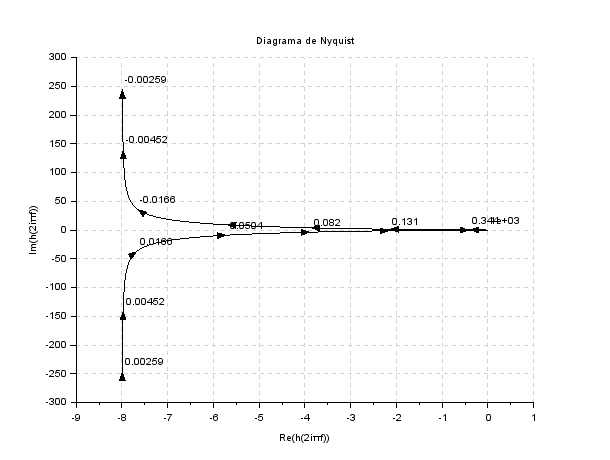
\includegraphics[width=7.75cm]{images/metodo_frequencial/plant_nyquist.png}  
        \label{nyq:freq:a}
    }
    \subfigure[Planta + PD]{                                              
        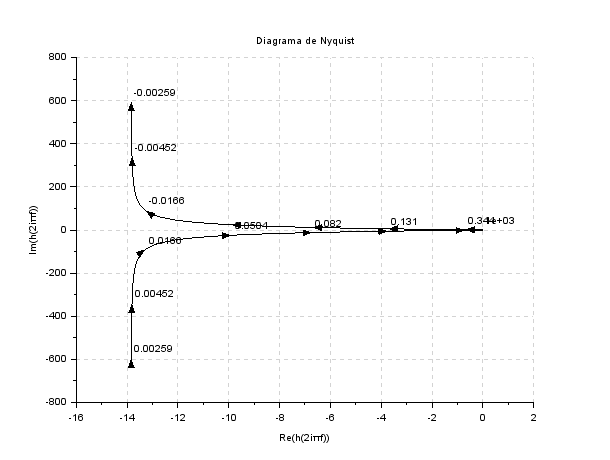
\includegraphics[width=7.75cm]{images/metodo_frequencial/plantPD_nyquist.png}
        \label{nyq:freq:b}
    }                
\end{center}
\caption{Diagramas de Nyquist obtidos no scilab com a função \textbf{nyquist()}.}
\label{nyq:freq} 
\end{figure}


De forma complementar aos diagramas de Bode obtidos com a função \textbf{bode()} e dispostos na figura \ref{bod:freq}, tanto para a planta sem controlador (figura \ref{bod:freq:a}), quanto para a planta com o PD (figura \ref{bod:freq:b}), também foram utilizadas as funções \textbf{p\_margin()} e \textbf{g\_margin()} para avaliar as margens de estabilidade dos sistemas. 

A função \textbf{p\_margin()} recebe como argumento a função de transferência e retorna a margem de fase (MF) e a frequência de cruzamento de ganho (fcg), sendo esta última comumente aproximada ao valor da frequência de corte do sistema. Já a função \textbf{g\_margin()} recebe como argumento a função de transferência e retorna a margem de ganho (MG) e a frequência de cruzamento de fase (fcf), sendo esta última comumente aproximada ao valor da frequência de corte do sistema.

\begin{figure}[H]
\begin{center}
    \subfigure[Planta]{             
        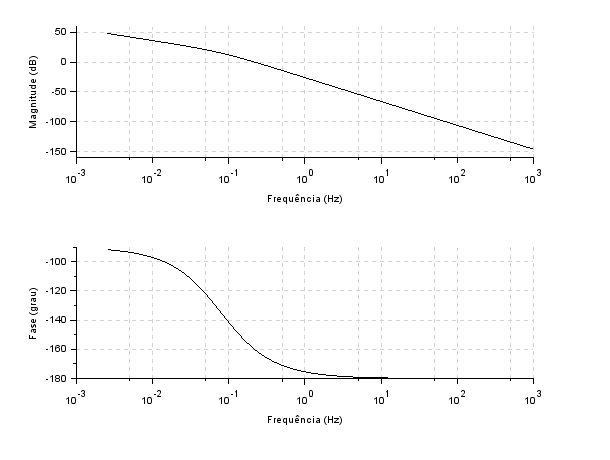
\includegraphics[width=7.75cm]{images/metodo_frequencial/plant_bode.png}  
        \label{bod:freq:a}
    }
    \subfigure[Planta + PD]{                                              
        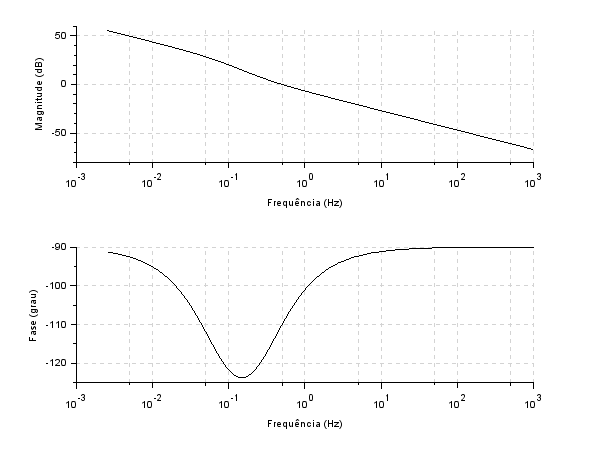
\includegraphics[width=7.75cm]{images/metodo_frequencial/plantPD_bode.png}
        \label{bod:freq:b}
    }                
\end{center}
\caption{Diagramas de Bode obtidos no scilab com a função \textbf{bode()}.}
\label{bod:freq} 
\end{figure}

Para o sistema da planta sem controlador obteve-se uma margem de fase de $20^{\circ}$ e frequência de cruzamento de ganho de $1.37 rad/s$, margem de ganho infinita e frequência de cruzamento de fase indefinida.

Já os resultados para a planta com o controlador PD obteve-se uma margem de fase de $70^{\circ}$ e frequência de cruzamento de ganho de $3.14 rad/s$, margem de ganho ainda infinita e frequência de cruzamento de fase indefinida. Dessa forma obtendo-se os valores assim como esperado no projeto.


\paragraph{XCOS}

No XCOS as análises foram feitas em um intervalo de tempo de 10 segundos, com tempo de inicialização em zero e período de 0.01 segundos.

Os parâmetros do PID utilizado na simulação são tais que obedecem a figura \ref{xcos:pid}

\begin{figure}[H]
\begin{center}
    \subfigure[Diagrama de blocos]{             
        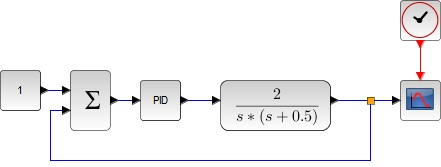
\includegraphics[width=6cm]{images/metodo_frequencial/xcosCL_PD.jpg}  
        \label{xcos:clpd:a}
    }
    \subfigure[Simulação temporal]{                                              
        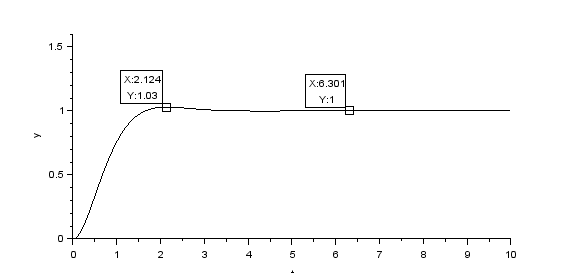
\includegraphics[width=9.5cm]{images/metodo_frequencial/timeCL_PD.png}
        \label{xcos:clpd:b}
    }                
\end{center}
\caption{Simulação no XCOS para a planta em malha fechada e com PD.}
\label{xcos:clpd} 
\end{figure}

\begin{figure}[H]
\begin{center}
    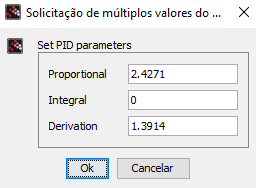
\includegraphics[width=5cm]{images/metodo_frequencial/pid.png}  
\end{center}
\caption{Parâmetros do controlador PID utilizado na simulação do XCOS.}
\label{xcos:pid} 
\end{figure}

Uma vez que o objetivo desse projeto é obter parâmetros no domínio da frequência, se faz necessário obter uma relação entre as medidas no domínio do tempo com os da frequência. Por sua vez, a margem de fase (MF) e o coeficiente de amortecimento ($\xi$) estão diretamente relacionados, de forma que: $MF = 100\xi$ (OGATA, 2009). 

Dessa forma, como já é conhecida pela literatura uma relação entre o coeficiente de amortecimento e o percentual de overshoot (OS), pode-se utilizar a equação \ref{mf} para relacionar diretamente a margem de fase com o pecentual de overshoot, já que o overshoot pode ser facilmente encontrado pela parcela do sobre sinal: $OS = \frac{c_{max}-c_{final}}{c_{max}}$

\begin{equation} \label{mf}
MF = 100\frac{-ln(OS)}{\sqrt{\pi^2+ln^2(OS)}}
\end{equation}

Dessa forma, da figura \ref{xcos:ma} conclui-se que a planta em malha aberta é instável. Já em malha fechada é estável na figura \ref{xcos:mf}, porém com oscilações e um percentual de overshoot de 36.26\%, implicando em uma margem de fase de $30.72^{\circ}$. Para o sistema em malha fechada e com PD, obtém-se um percentual de overshoot de 3\%, implicando em uma margem de fase de $74.75^{\circ}$, assim como o esperado pelo projeto.

Dessa forma garante-se a veracidade do controlador para garantir os parâmetros de desempenho desejado, permitindo avançar para a aplicação prática do circuito.

\pagebreak